\documentclass[11pt, oneside]{article} 
\usepackage{geometry}
\geometry{letterpaper} 
\usepackage{graphicx}
	
\usepackage{amssymb}
\usepackage{amsmath}
\usepackage{parskip}
\usepackage{color}
\usepackage{hyperref}

\graphicspath{{/Users/telliott/Github/calculus_book/png/}}
% \begin{center} 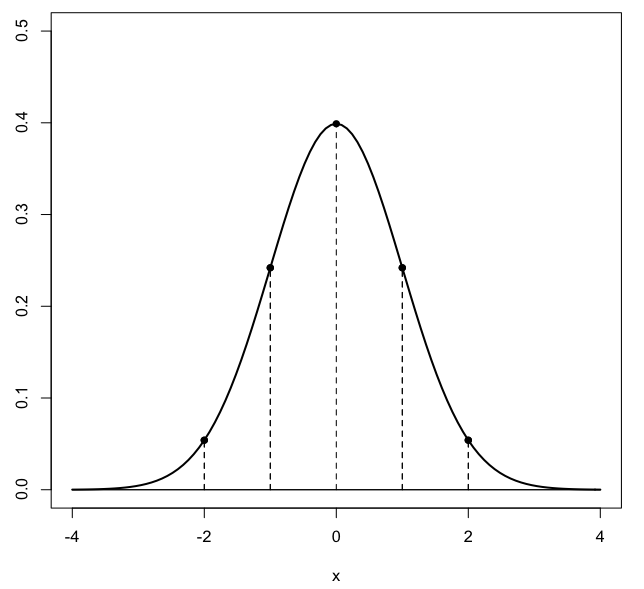
\includegraphics [scale=0.4] {gauss3.png} \end{center}

\title{Basic number theory}
\date{}

\begin{document}
\maketitle
\Large

The next two chapters don't have a lot to do with calculus, but are here to show some key results of Euclid.  One is the Euclidean algorithm, and another is the Fundamental Theorem of Arithmetic.  Though he never stated the fundamental theorem in its modern form, Euclid had all the pieces figured out.  

It shows some more sophisticated but not too challenging proofs.  

This can be skipped without interfering with the development of the rest of the text, except that the fundamental theorem is used in the chapter on irrationals to greatly simplify two proofs about irrational numbers.

\subsection*{Euclidean algorithm}
Consider 2 natural numbers $a$ and $b$.  Usually $a$ is allowed to be an integer (i.e., it can be negative), but here we will say that $a,b \in \mathbb{N}$, $a$ and $b$ are positive integers.

We can find their \emph{greatest common divisor}, written $(a,b)$.  Here's an example:

\begin{verbatim}
180 =          2 x 2 x 3 x 3 x 5
140 =          2 x 2 x         5 x 7
gcd(140,180) = 2 x 2 x         5 = 20
\end{verbatim}

First we write the unique prime factorization of $a$ and $b$ (see below).  Then pick out the common factors and the gcd$(a,b)$ will be their product.  It is important that we do not need to actually factor $a$ and $b$.

The algorithm works like this:

$\circ$ find integers $r \ge 0$ and $q > 0$ such that

\[ a = b \cdot q + r \]

If $r = 0$ we are done:  $b$ divides $a$ equally.  Otherwise

$ \circ$ switch $a = b$ and $b = r$ and repeat.

Then $b$ is the gcd of the original $a$ and $b$.  In our example

\begin{verbatim}
180 = 140 x 1 + 40
140 =  40 x 3 + 20
 40 =  20 x 2 + 0
gcd =  20
\end{verbatim}

Here is the reason this works.  First, we can always find $q$ and $r$ such that
\[ a = b \cdot q + r \]
\begin{center} 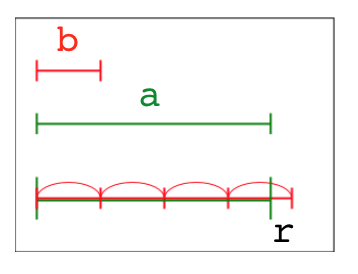
\includegraphics [scale=0.4] {Archimedean_property2.png} \end{center}

Proof:

$\circ$ Either 
\[ a = b \cdot q \]

$\circ$ Or
\[ b \cdot q < a < b \cdot q + b \]
So then
\[ a - bq > 0 \]
\[ a - bq < b \]
and we set $r = a - bq$.

So then let $u$ be the largest integer that divides both $a$ and $b$

\[ a = su \]
\[ b = tu \]
Then 
\[ su = q \cdot tu + r \]
\[ r = su - q \cdot tu \]
\[ r = u(s - q \cdot t) \]
So $u$ divides $r$.

Hence every common divisor of $a$ and $b$ is also a divisor of $b$ and $r$.

There is much more developed in the \emph{extended} Euclidean algorithm that is useful for cryptography.

\end{document}